
%No description of the act is complete without a description of the act of Majlis al-Aza’ and the \emph{mūkeb} procession. While both rituals are public and allow for anyone to join in, majlis al-aza’ is ultimately performed for a wider audience, where as the \emph{mūkeb} processions are performed for Karbalaeis themselves. 

% Neither ritual is limited to Karbala. While the majlis is performed all across the world in Shi'a communities, the \emph{radat}s are limited to the shrine cities in Iraq, around Imam Askari, Imam al-Hadi, Imam al-Kathim, Imam al-Ridha, Imam Ali, and Imam Hussein. It is unclear whether \emph{radat}s are performed around Imam Reza in Mashad, and such rituals are not practiced around the tombs of the Imams in Saudi Arabia. It is for this reason that the rituals are less discussed in modern studies of Shi’a rituals, but this does not make them any less important. 

% chapter 2 points:
% - bureaucratic representation is mixed in with tribal representation
% - neat history of karbala
% - religious rituals are fraught for clerics 
% - what's really interesting is the repetition and oral history with opens traditions to changing, eating away at the clerical class

In 2017, nearly every tribal leader within Iraq outside of the Kurdistan region gathered in Karbala to sign the Karbala Honor Pact. Passed in response to a push by the government to crack down on tribal violence, the Karbala Honor Pact was issued on May 23rd, 2017, co-signed by tribal leaders, the Directorate of Tribes within the Iraqi Ministry of Interior, and the Karbala Center for Shi'a Studies. The Honor Pact specifies 14 points, all of which aim to reduce violence between tribes, such as outlawing forced displacement of tribes, reprisals against medical staff when a patient dies, rejecting collective punishment of families, and so on. In particular, the tribal custom of \emph{degga} was rejected, a practice that involved targeting one party's house within a conflict with weapons such as guns and grenades in order to force them into the negotiating table. 

This process largely mirrors the changes of tribal policies to north Iraq as well during the same period. The post ISIS environment, which has yet to be filled by government authority, has lead to an expansion of other authorities, such as the Hashd. While the Hashd have filled the security vacuum, the lack of a functioning judicial system and widespread corruption in state authorities have lead scholars to note the role tribal mechanisms such as \emph{bara'a}, \emph{tabri'yya} and \emph{kafala} have played in reintegration of families that have been associated with ISIS \cite{genat_state_nodate}.

Tribal influence within Iraq is deeply built into the system, and Karbala is no different. As tribal influence predate clerical influence within the area, the oft-repeated perception of Karbala as a Shi'a city requires reexamining. In my view, many of Karbala's practices are actually more tribal than they are Shi'a Islamic, even as the two have aligned on particular ideals. Nothing is more exemplary of this role than the role of \emph{muwālkib}. 

\section{\emph{Mūkeb}}
A \emph{mūkeb} functions as the fundamental unit of organization for Shi’a rituals within Karbala. While not deemed specifically a Husseini ritual, the \emph{muwālkib} are responsible for organizing and providing services in order to facilitate the Husseini rituals. Villages around Karbala are typically organized alongside somewhat fluid tribal lines, the urban nature of Karbala removes the tribal division. Instead, Karbalaeis organize themselves along \emph{beiyūtat} (\begin{Arabic}بيوتات\end{Arabic})\footnote{This is already a double plural, \begin{Arabic}بيت\end{Arabic} is the singular form of the word "house", \begin{Arabic}
    بيوت
\end{Arabic} is the plural form of "houses. In order to distinguish the specific nominal meaning of "houses" or "clans", the Karbalaies have added the feminine plural ending of \begin{Arabic}
    -ات
\end{Arabic} onto a masculine plural word, forming \begin{Arabic}
    بيوتات
\end{Arabic}}, or houses. These houses often group together to form \emph{muwālkib}. The \emph{muwālkib} collect money from the affiliated houses and solicit outside donations in order to provide services for pilgrims, which religious devotees see as part of their duty to provide. 

\emph{Muwālkib} can also be from larger neighborhoods, such as the seven great \emph{muwālkib} of Karbala, explained later. The Hashd al-Shaabi also provide \emph{muwālkib} along the road from Najaf to Karbala. The manager of the Department of \emph{Muwālkib} describes this as:

\begin{quote}
    Anyone can start a \emph{mūkeb}...if someone wants to start a \emph{mūkeb} because they want to serve fish instead of lamb, they can go down the street and start a second [\emph{mūkeb}]. It is only in the city that we enforce licenses, because there is not enough space.
\end{quote}

A key function of the \emph{mūkeb} is to provide services for pilgrims in a tent. The term \emph{mūkeb} is used for both the tent and the organization itself. The tents can range from a single small tent with a stall providing basic food such as cheese and bread, to a full service tent providing sleeping space, cooked food, air conditioning, electricity, medical care, and foot massages. Many larger mokwebs also provide space for rituals to be performed, although this may overlap with space that a \emph{husseiniyya} provides. It is not uncommon to see a \emph{husseiniyya}'s courtyard be filled with a particular family's \emph{mūkeb}, which provides food and other services. 

During the day before Ashura, as well as the week leading up to Arbaeen, the area around the two shrines is filled with \emph{muwālkib}. The Department of Muwalkib, run by the shrine of Abbas, is responsible for providing licenses and other various logistical efforts in supporting \emph{muwālkib} around the city. 

\subsection{Schools of Thought (Shirazi, Iranian, Qaziwini, etc)}
Among the many \emph{muwālkib} are the different schools of thought. Each \emph{mūkeb} is affiliated with not only a particular neighborhood, but the traditions of the neighborhood itself influences the political nature of rituals. For example, on the Qibla road leading towards the Shrine of Imam Hussein, multiple mokwebs can be see bearing the pictures of Ayatolla Sadiq Shirazi. Another popular \emph{mūkeb} is run by the family of Ayatollah Qazwini, which runs Husseiniya Qazwini, whose popularity in the United States has helped popularize the \emph{mūkeb} itself. 

The \emph{muwālkib} are highly political as well, with many affiliated with the Hashd al-Shaabi. Opinions of the Hashd range from them being Iranian proxies to defenders of the faith, with many \emph{muwālkib} along the road creating mock graves for Abu Mahdi Muhandis and Qassem Soleimani. 

\subsection{The Seven Great \emph{Muwālkib}}
Although \emph{muwālkib} function as a unit of organization, the seven great \emph{muwālkib} have grown to encompass entire neighborhoods. Originally the seven neighborhoods surrounding the shrines of Karbala, each has developed into a distinct neighborhood with its personalities \ref{fig:mowalkib} in the old city. During my fieldwork, I walked with a member of each neighborhood in order to map out the boundaries on each \emph{mūkeb}. During Muharram, members of each neighborhood typically gather into their specific \emph{mūkeb}, with each \emph{mūkeb} performing a procession between the shrines of Imam Hussein and Abbas. In clockwise order they are:  Mukeb Taraf Bab Baghdad, Mukeb Bab al-Khan, Mukeb Taraf Bab al-Najaf, Mukeb Taraf Bab Abasiyya, Mukeb Taraf Bab al-Mukhaym, Mukeb Taraf Bab al-Taq, and Mukeb Taraf Bab al-Salam.

\begin{figure}
\caption{The seven great \emph{muwālkib} of Karbala. Exact neighborhood streets are subject to change occasionally, these represent the rough boundaries on each \emph{mūkeb} neighborhood. Map made from author's fieldwork.}
\centering
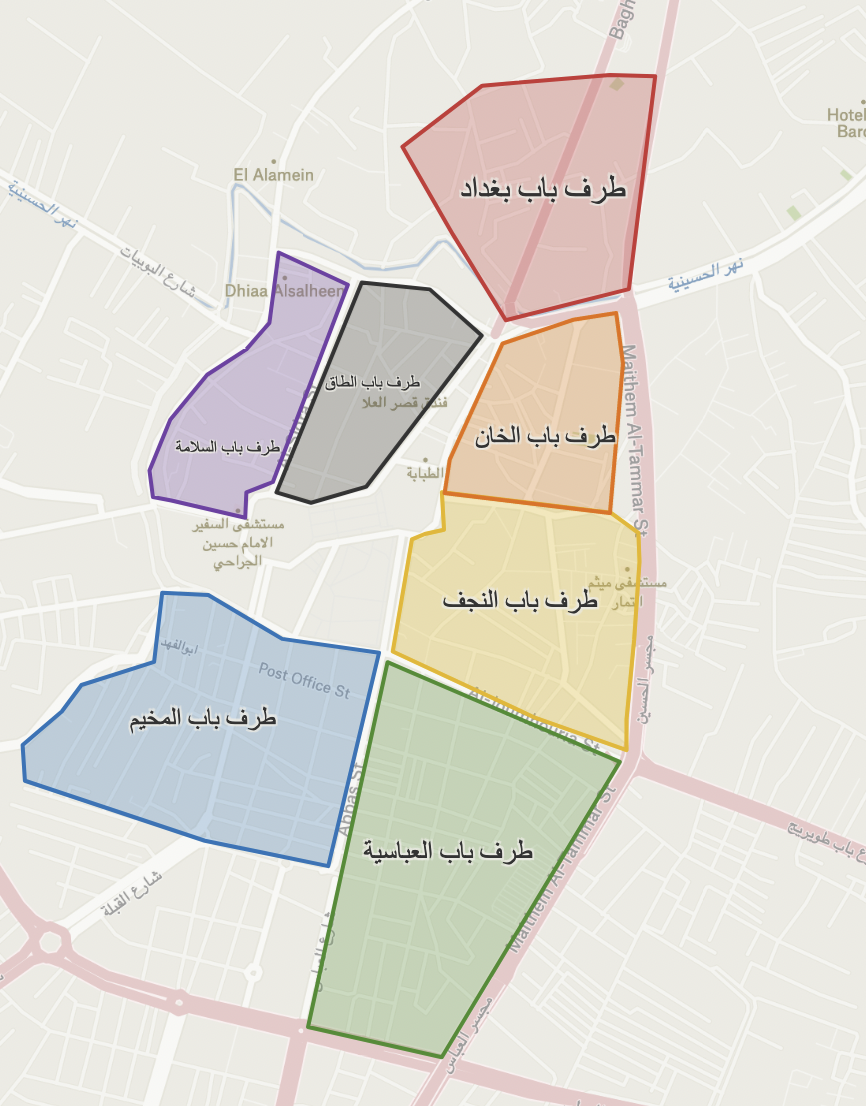
\includegraphics[width=0.5\textwidth]{images/seven-mowkebs.png}
\label{fig:mowalkib}
\end{figure}

As each of the seven great \emph{muwālkib} trace their roots to the founding of Karbala, their boundaries has been built into the roads of the city. The major highways leading to Baghdad and Najaf were built around the \emph{mūkeb}-neighborhoods themselves, leaving a the \emph{mūkeb} divisions within the architecture of the city itself. 

Mukeb Taraf Abbasiyya is the most politically active \emph{mūkeb}, with many interviewees claiming that they are "communist". While it is unclear how many communists actually resided in the neighborhood or were affiliated with the mokweb in the neighborhood as local records are not clear, the \emph{mūkeb} procession of Taraf Abbasiyya is known to be more political than the others, especially \emph{radat}. 

\section{\emph{Radat}}
A special ritual is conducted by the seven great \emph{muwālkib}, known as Radat Siyasi Karbalaei. Each \emph{radat} has 3 distinct parts: the banner, the \emph{howdej}, and the chant itself. 

The banner announces which \emph{mūkeb} the procession is affiliated with. The banner is an ornately decorated banner, held by two men, which spells out “\emph{mūkeb} X” in Arabic. Oftentimes this is accompanied by flags afterwards, which may be Iraqi flags, flags relating to Shi'a Islam, or flags of various Islamic colors. Multiple \emph{muwālkib} had flags bearing “Ya Hussein” or the Iraqi flag itself, which presents an interesting contrast of nationalism and religion. 

Following the flags is usually the \emph{howdej}: a 70 kilogram boat that is often carried by a single man \ref{fig:howdej}. A hadith from the prophet described Imam Hussein as the light of salvation, leading Shi'as to construct a metal boat of lamps. Either electric or gas-lit, the \emph{howdej} is a mainstay of Shi'a rituals between the third of Muharram to the ninth of Muharram. Cries of mourning can be heard as they carry the \emph{howdej}, with subsequent chants of "ya Allah!" or "ya Ali!". The \emph{howdej} itself is adorned with lights in the shape of a pyramid, crowned with a wreath at the top, representing Hussein. Two snake-like creatures flank the ends of the ship, with their open mouths turned towards the pyramid of light, representing the evil that lurks and the danger the world bears towards Hussein. 

\begin{figure}
    \centering
    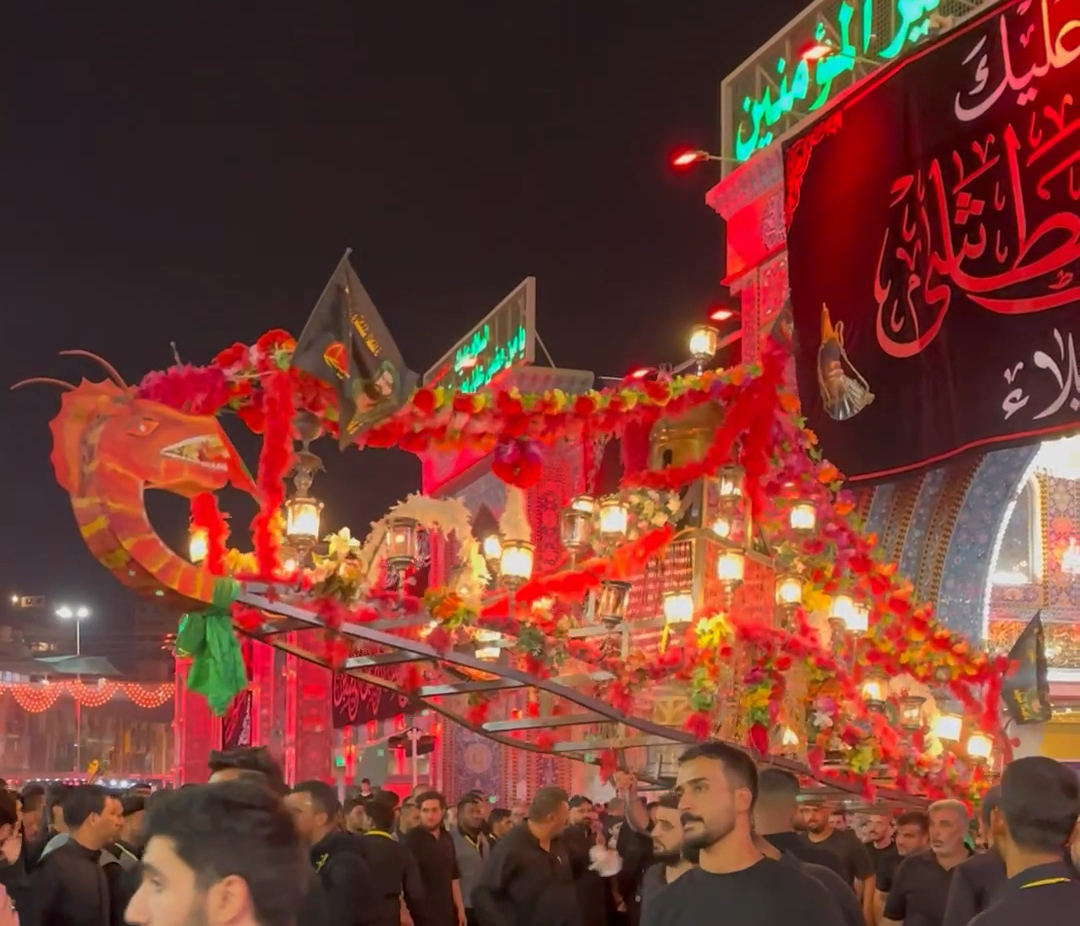
\includegraphics[width=0.5\textwidth]{images/howdej.jpg}
    \caption{A \emph{howdej} being carried from the shrine of Imam Hussein. Note the snakes emerging from both ends. Image taken by author on August 5th, 2022.}
    \label{fig:howdej}
\end{figure}

% \begin{figure}
%     \centering
%     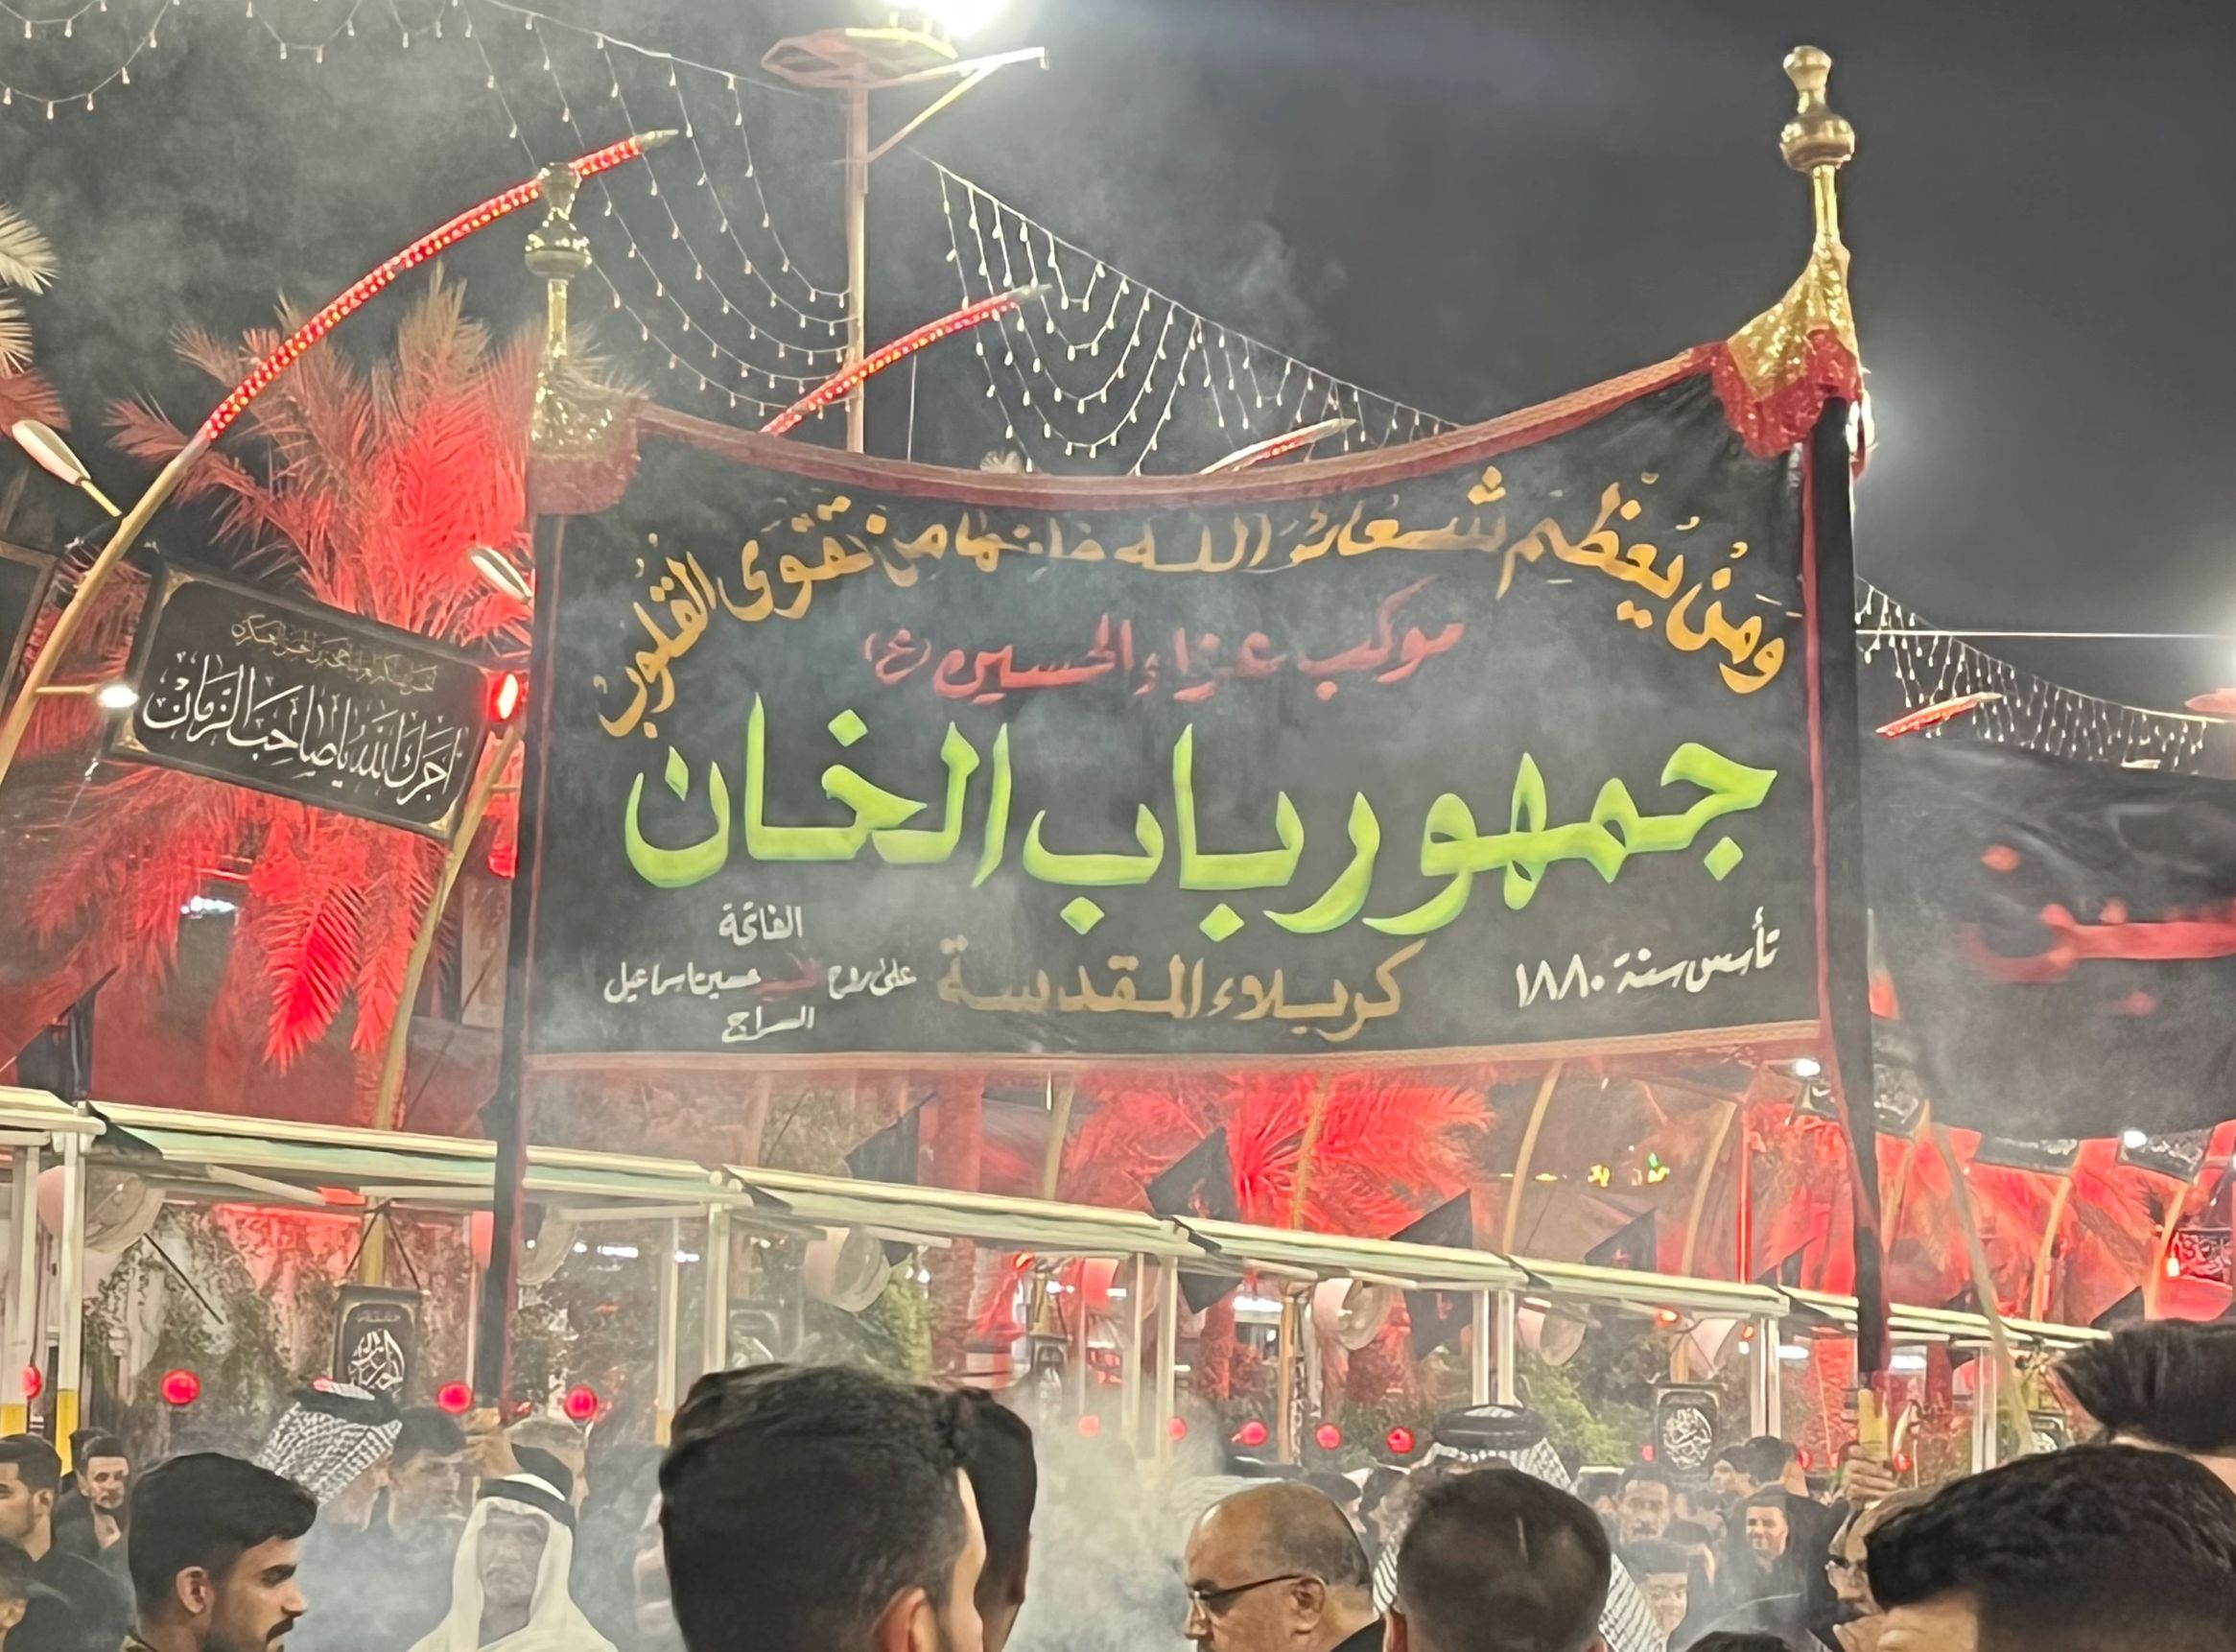
\includegraphics[width=0.5\textwidth]{images/mowkeb-bab-alkhan.jpg}
%     \caption{The banner of \emph{Bab al-Khan} procession. Image taken by author on August 4th, 2022.}
%     \label{fig:bab-alkhan}
% \end{figure}


Following the \emph{howdej} is the main part of the \emph{radat}: the chants themselves. A member of the mokweb, usually a young man, holds a sign and leads a group in chanting. There can be any number of groups, usually ranging from 5 to 10, with each group chanting a section of the poem. Men join and leave groups as they like, but usually due to how crowded the area between the two shrines is, members usually stick with one group, chanting the same three lines and the refrain as they begin at the gate of Abbas, through the Abbas shrine, through bayn haramiin, and through the shrine of Imam Hussein. 

Walking with all seven great \emph{muwālkib}, I noticed that the chants were around various different topics. While one of my interviewees mentioned that, in previous years, chants were around the electricity services, or water services in the city, the chants from 2022 were largely centered around Shi'ism or Iraqi Nationalism. One \emph{mūkeb} in particular, Mukeb Taraf Abassiyya, is famously political in their \emph{radat} chants. One of their chants stated: 

\begin{quote}
\begin{Arabic}
جيران الوطن كلهم أفاعي

علي أتامروا فرهدوا كاعي

كل العالم يشوف

بكاعي الطامع يحوف

يحسين انت رايه

الحق هداية
\end{Arabic}
\end{quote}

Translated as: 
\begin{quote}
All of the neighbors of the homeland are snakes

Against me, they conspire to steal my land

The whole world sees

The thieves which roam my land

Oh Hussein you are the banner, the true guide
\end{quote}

On first observation, what stood out the most was the usage of "\emph{waṭan}". Watan colloquially refers to a homeland or nation. Initially, I thought the usage of "\emph{waṭan}" within this \emph{radat} may have referred to an ambiguous Karbalaei conception of \emph{waṭan}, or even a Shi'a \emph{waṭan}, but every person I asked this question refuted this understanding, and stated that \emph{waṭan} refers to Iraq in its modern nation-state form. Taken this, the phrase “neighbors of the homeland” then refers to the current political events occurring between Turkey, Iran, and Iraq. 

This stands in contrasts to my interviewees in Baghdad and other cities, who often claimed that the Karbalaei’s are “Iranians in origin”. When I visited \emph{Wadi Salaam} and spoke with some gravediggers about the graveyards in Karbala, many them mentioned that the Karbalaeis have different politics than Najafis because the area was “settled by Iranians”. 

The contrast between how the Karbalaeis are perceived vs how they see themselves is striking: while they are perceived as foreigners in the state of Iraq, the Karbalaeis themselves see themselves as representative for Iraq, making competing claims to unity. While the usage of the Iraqi flag during rituals may be seen in a sectarian light, such as Shi'as laying claim to the state and the nation, The \emph{radat} provides additional depth. By claiming the neighbors of the \emph{waṭan} are snakes, the Karbaleis are carving a different path beyond simple sectarianism, they are making a claim to a particular form of unity that incorporates that deeply incorporates the conceptions of the nation-state, in contrast to the ideas about the "Shi'a crescent" \cite[120]{haddad_understanding_2020}. 

The \emph{radat} chants also present themselves as an interesting intersection of the political, the religious, and class. Rather than seeing these spheres as disparate spheres, the Karbalaei’s themselves easily mix these together, with the conceptions of the nation-state interacting with the fact that the ‘ulema do not participate in these chants. There is a special \emph{mūkeb} called Mukeb Imam Hussein which is affiliated with the workers and members of the Shrine of Imam Hussein, but this \emph{mūkeb} is not affiliated with any traditional neighborhood. The overriding notion is not politics or sectarianism, but rather a distinction within the religion between the language, between the religious educated and the rituals of the streets. What is more interesting is that the \emph{radat} chants are a purely oral tradition, upon asking various historians and poets affiliated with different \emph{muwālkib} and the shrines, the tradition is strictly oral. To the best of my knowledge, despite looking in the archives at the Center for Karbala Studies and the archives in the Karbala Central Library as well as various bookstores around town, I may be the first person to draw a map and record \emph{radat}s in recent history. The \emph{radat}s conducted by the Karbalaeis are avowedly present in nature and similar to majlis: the chants are about current events, or past events drawn into the present, while their oral nature allows them significant room to change: the past is malleable because it is not conducted in MSA, and conducted in the tongue of the people. 

\section{\emph{Tatbir}}
Ashura, the 10th of Muharram, begins at dawn. I had slept at a \emph{husseiniyya} near the Shrine of Imam Hussein the night before in order to witness the event in its entirety. The \emph{husseiniyya} was already packed with pilgrims when I arrived the night before, I found a small cot near the wall and napped for a few hours. At 3:30am, I stumbled over to the Qibla road, the road that terminates at Bab al-Qibla in the shrine Imam Hussein. When I arrived, the celebrations were already in full swing. A throng crowded the streets, with soldiers and policemen attempting to divert the sea while maintaining distance from the people. The main event was about to begin, with the focus on \emph{tatbir}. 

\emph{Tatbir} is the practice of ritualized bloodletting. Shaving of the head, followed by cutting of the flesh, either through quick, repeated strikes or a swift incision on the surface of the skin is made. \emph{Tatbir} is religiously controversial, even among the Shi'a, Ali Khamenei forbids \emph{tatbir}, Ayatolla Sistani has never given a fatwa on it, and other opinions of the clerics range from completely forbidding it, to allowing it under special circumstances, to encouraging it as a mustahab act. The Iraqi Shi'i \emph{mutjahid} ‘Abd al-Husayn al-Hilli has argued that the formation of these \emph{tatbir} and other ritual lamentations have become public events in recent years, but notably only mentions weeping and beating of the chest as religious obligations \cite[85]{weiss_shadow_2010}, with \emph{tatbir} conspicuously absent from his rulings. Theological debates aside, the International Media Department of the Shrine of Imam Hussein attempted to bar me from taking photos of \emph{tatbir} in previous discussions, although such a rule was impossible for them to enforce. 

Dressed in white to showcase their bleeding, I saw a massive crowd march towards the gate of Imam Hussein, all men of various ages. I saw a young boy with a shaved head, no more than ten years old, walk up to an elder, offering the older man a small kitchen knife. The elder man made a swift and precise incision at the base of the skull, drawing blood, and offered the boy a white cloth to gather the blood. Other men held large swords, repeatedly vertically striking themselves on their skull with repeated shouts of "Haider!", another name for Imam Ali. From the second floor of the shrine, I could see women pressed against the window, watching the men. Cottons swabs soaked in iodine were handed out from various volunteers to sterilize the \emph{tatbir} wounds. A shocking amount of blood flowed in the streets with the mass of people making it impossible to move freely. Pushed around by the crowd, my sandals became stained in blood. Other spectators pressed their kuffiya or their shirts against their face to prevent themselves from vomiting. The air reeked of blood, iodine, and sweat. 

As the crowd pushed me towards Qibla gate, I saw the participants cry out and raise their blades towards the sky. Drums and trumpets blaring, they marched into the shrine as I ducked out from under some swords.

Like \emph{radat}, \emph{muwālkib} arrive in procession to perform, although instead of black banners, the \emph{tatbir} ones utilize white banners and red text, mimicking blood, playing a similar role to \emph{radat}s. However, the key difference is the hemic element, cutting of the head and bleeding is meant to evoke an imagery of sacrifice and justice. Edith Szanto has written about \emph{tatbir} in the context of the Damascus, noting how women were particularly proud of their husbands for participating \cite[86]{szanto_beyond_2013}. In a similar way, \emph{tatbir} in Karbala provides the same: I witnessed a young boy, no more than 8, having his head cut open by an elder. Afterwards, the entire \emph{mūkeb} gathered and congratulated the boy for his first \emph{tatbir} experience. The \emph{tatbir} experience a literal sublimation of the self via blood which then binds people together\footnote{Blood brother style rituals are similar to \emph{tatbir}. In Iraq, another tribal practice is called Kriev, which is similar to a blood brother ritual, but serves to bind two families. Kriev is a circumcision ritual, a boy of a weaker family is circumcised in the lap of the patriarch of another, more locally powerful family. Krievs were conducted between Yazidi families and Arab families before ISIS, however, many Yazidis have turned against the process, as many were given up to ISIS when they sought protection from their kriev families. It is unclear to me where the origins of the Kriev are, I have interviewed non-Yazidi Kurds with Kriev families all over northern Iraq. The practice seems less common in the south, however.}. 

\section{Services}
The most visible role of \emph{muwālkib} for pilgrims is during Ashura and Arbaeen, where \emph{muwālkib} provide services such as food, water, and places to rest. \emph{Muwālkib} will setup tents, with the numbers ranging from one to many, offering a dizzying array of services, such as medical care, bathrooms, foot massages, cooked food, areas for rituals, and so on. Other \emph{muwālkib} offer memorial services, such as many Hashd \emph{muwālkib} providing a museum for viewing propaganda as well as museums of war memorabilia for fallen martyrs of the Hashd. During Arbaeen, I walked through a \emph{mūkeb} which featured a cardboard cutout of both Qassem Soleimani and Abu Mahdi Muhandis, two men who were killed by the United States in early 2021. As both men were key figures in the militia regime between the Hashd al-Shaabi and the Iranian Republican Guard Corps, this \emph{mūkeb} offered a chance for pilgrims to see mock graves and take photos with their respective uniforms. 

Iraqis residents raise money throughout the year in order to provide these services, including soliciting donations from the local community and around the world if they have additional resources. With innumerable service \emph{muwālkib} during every ziyara, an immense amount of resources is poured in, from furniture to cleanup to raw food material.

Many of my interviewees pointed out the inclusive nature of service \emph{muwālkib}, with service \emph{muwālkib} being run by Lebanese, Iranians, Bahranis, and so on. The walk between Najaf and Karbala is approximately 80 kilometers, and the unit of measurement is electrical poles, which span every 50 meters. Pilgrims during the walk refer to specific \emph{muwālkib} near different poles as identification. Near pole 596, I saw a \emph{mūkeb} being run by Thailand Shi'a, who had a large banner written in Thai mentioning that it was the eighth time this group of Thailand Shi'a had done this. 

Lale Can has written about the Sufi culture of guest lodges for pilgrims, which provided similar services and served as institutions of learning for Sufi pilgrims travelling to Mecca and Medina \cite{can_spiritual_2020}. Can noted that these lodges existed in precarious positions with regard to the Ottoman state authorities that managed pilgrimage, with fears from state authorities that pilgrims would overstay their welcome by living the the guesthouses for an extended period of time. The tension between the Ottoman Empire's role as a Muslim empire competed against the state imperative of control of guests via passports. As Christopher Low describes, the Ottoman Empire was deeply concerned about the rise of Indian immigrants to Mecca and Medina and how the empire authorities saw them as British subjects, and therefore a play by the British to assert control over the Hijaz \cite{low_imperial_2020}. 

These tensions of state needs and religious needs continue today, albeit in slight different forms. The key difference in that Sufi guest lodges usually were attached to a specific mosque or waqf. Shi'a \emph{muwālkib} can be affiliated with any group, whether that group is a specific militia, homes or group of homes, or even individuals. Inside city limits of Karbala, especially closer to the shrines, \emph{muwālkib} require a license, which are issued through the al-Kafeel Department of \emph{Muwālkib} near the Abbas shrine. However, outside city limits, especially on the road from Najaf to Karbala or Baghdad to Karbala, \emph{muwālkib} are effectively unregulated, anyone can place a \emph{mūkeb}, start \emph{mūkeb}, collect donations for one, and so on. 

The sheer number of \emph{muwālkib} only complicates the relationship they have with the state. The Iraqi visa regime is complex and often confusing, a brief discussion with the Thailand Shi'a revealed that the religious visa, which is intended to offer 30 day stays for pilgrims, is often not enough time to sufficiently prepare, such as organizing logistics around food, electricity, and generators. As Muharram has shifted into the summer months, air conditioning in \emph{muwālkib} has become a necessity, despite the fact that the electrical grid continues to deteriorate whenever summer arrives in Iraq. Karbalaeis mentioned on multiple occasions of the negative view towards Iranians, specifically the stereotype of Iranians as freeloaders who come to Iraq only to demand free food and lodging, while throwing trash everywhere and providing nothing in return. 

One key point that was repeated is that the Iranian pilgrims arrive in Iraq without a passport. During normal conditions in Iraq, there are checkpoints between every governorate, as well as within Baghdad itself, and before specially closed areas. Iraqis and foreigners grow accustomed to these checkpoints, with the checkpoint police often being the butt of jokes as uneducated and illiterate. In addition, these checkpoints are not only run by the state, they are run by a variety of militias and local groups. For example, the checkpoint into the city of Samarra is run by Sayara Salaam, or Peace Bridages, the successor militia to Muqtada Sadr's infamous Jayesh al-Mahdi, while a checkpoint on the Jadriyah bridge in Baghdad, one of the major arteries of the city, is run by the Kurds. The formal legislation around checkpoints seems loose as well, crossing into different cities often requires two or three checkpoints, usually with a state checkpoint followed by one or two militia checkpoints. While these checkpoints have become routine to people's lives, they are also very serious, checkpoint police have unilateral power to arrest and detain anyone for an indefinite amount of time. For example, when attempting to cross into Samarra for the first time in 2021, I was arrested by the checkpoint police for "seeming suspicious" and thrown in jail for over 18 hours with other men who had been detained, some of whom had been in jail for months. The high stakes nature makes it such that every foreigner in Iraq, and even Iraqis, know that proper documentation is necessary, lack of proper documentation could result in major consequences. 

However, during Arbaeen, most Iranians arrive without a passport, crossing the Iran-Iraq border with only their Iranian ID's, and often without any money as well. The checkpoint between Najaf and Karbala is typically an array of concrete walls manned with soldiers, yet during Arbaeen I was shocked that it was completely unmanned. Pilgrims simply streamed through the checkpoint, and the only process resembling the feared bureaucracy was a simple, hurried patdown. The scale of pilgrims, and the sheer amount of services and lodging available from service \emph{muwālkib} meant that there was always more capacity for pilgrims, inducing demand. This overwhelmed state capacity, to the point where the state must partner with independent organs like the Hashd, who blare out propaganda images and videos of Hashd soldiers guarding the road. 

% - talk about the thai \emph{mūkeb} and international \emph{muwālkib}
% - talk about the perception of generosity and the role that \emph{muwālkib} play
% - raising chickens in the backyard and fattening them, the role of \emph{muwālkib} matter a lot for individual residents 
% - talk about the perceptions of Iranians 

% \section{Hosa}
% Hosa is a tribal ritual conducted by south Iraqis. Hosa consists of two to four people, engaged in verbal poetry. Similar to slam poetry or battle rap, hosa is rooted in tribal tradition. Spectators organize in a circle around the participants performing hosa, and draw a wide audience. A rural/urban split occurs as well, as urban south Iraqis do not perform hosa. 

% I first encountered hosa during the nights leading up to Arbaeen, where I saw it being performed in the streets around the shrine of Imam Hussein. After asking a few people, they described hosa as a tribal ritual, and not a necessarily Shi'a one. Hosing provided an interesting mix of local cultural traditions mixing with religious traditions: pilgrims, who had come to Karbala in order to perform visitations had brought their own rituals as well. This matches to the descriptions my interviewees had about various forms of latm from other non-Arab Shi'as: \emph{latmiyyat} from Pakistani Shi'as were described to be more violent, while \emph{latmiyyat} from Iranians were perceived to be quicker in pace. 

\section{Repetition in the Procession}
A key part of both rituals is iteration: both rituals draw in the participant and revolve around repetition. Hamid Dabashi has written about an Iranian Shi'a ritual called \emph{ta'ziyah}, a play similar to the Christian Passion plays. He specifically describes \emph{ta'ziyah} and Shi'ism as a constant mourning: "the act of remembrance will have to remain always incomplete-like a dream that keeps haunting a people, forcing them to try to remember it, but never successfully." \cite{dabashi_taziyeh_2005}. Repetition here serves as the basis for a certain type of harmonization between people, either in lieu of possession, or in some cases, actual possession. Through repeated chants, participants internalize specific states, either with the concept of tragedy or mourning. Through repeated symbols, each repetition moves recognizes the previous one, but adds new features. The \emph{mūkeb} procession is a key example of this.

As mentioned before, the \emph{howdej} is a heavy boat that begins every \emph{mūkeb} procession. Derived from the word \emph{howdej} in Arabic, meaning a bed carried by a camel, the \emph{howdej} is usually carried by one or two men during a procession. Shaped like a triangle, the \emph{howdej} is richly adorned with lamps and flags. The core of the \emph{howdej} is a metal pyramid structure, often bearing remarks related to Hussein. Lamps are placed symmetrically on each side of the pyramid, with a single lamp at the very top. There is significant variation in \emph{howdej}, with only the core structure being regulated. 

\emph{Howdej}, at the beginning, lacked the snake-like creatures that represented the coming evil against Imam Hussein. When asked, many residents of Karbala could not tell me when this feature as added, but recognized its symbolism. Latm and qasidas have similarly incorporated drums and other features throughout time, but retain their clear identity. The rituals have also taken on a showmanship identity, with individuals competing against one another, such as in the case of carrying the pillar on the head. 

Recognition is even more explicit, because of the overly public nature of the rituals. Building on that the rituals are recognized as \emph{husseiniyya} rituals, the public spectacle element of the rituals means that iteration happens faster than before, leading to new additions and changes. Another example of this is the flag changing ritual, where the flags are pulled down and changed before Muharram. This ritual began in 2006 \cite{hamdan_development_2012}, and is extremely conspicuous, as the flag and domes of Karbala are omnipresent in the imagery. 

It is impossible to attend a majlis or \emph{radat} that is not photographed, videotaped, or livestreamed in Karbala. The holy nature of the city means that visitors are encouraged to videotape, but because rituals participants recognize themselves and others within the photograph, they are encouraged to compete and iterate, not only with their peers, but with their past selves. The photograph, as Johnson states: "mediates a scene or person in a place and time different from those in which the photograph is viewed and the here and now. The quality of being at once an image and a thing is important because it enables the photographs’ multiple lives, crossing dimensions" \cite[92]{johnson_automatic_2020}. Photographs and videos are not a side-effect on the ritual, which pushes it forward, but rather a part of the ritual itself. In the same way the latm draws in the participant by encouraging them to chant, \emph{husseiniyya} rituals in general encourage participation through videotaping. The rituals are not spectacles that get photographed, they are spectacles because in order to encourage photography. 

\section{Photography and Language}
One curious practice I saw was bringing people virtually to Karbala by dialing a video call or pulling up a photograph, placing the person’s image upon the background of the shrine, and using a second phone to take a photo. I saw men using a Whatsapp video call, then placing their mother’s face in the phone against the backdrop of Bab al-Qibla of the Shrine of Imam Hussein. Similar photographs abound on social media, where they are endlessly reposted \footnote{https://twitter.com/JawadAbubakar7/status/1570739286873612290}. Similar to the explicit rituals, the end result of this is a photograph of a person and the shrine, showing that the photograph generation holds the key here. 

During a casual conversation with my neighbor, he mentioned how the \emph{howdej} had changed very quickly within the last few years, including sprouting snakes at each end of the boat. Marching with \emph{howdej} is also a very public ritual, ritual participants are eager to show that they can carry a \emph{howdej} by themselves. Cries of "mashallah" surround the bearer as they are recorded, shared, and re-shared along social media. 

Combined with the common practice of carrying around two smartphones in Iraq\footnote{This is due to various issues with cellular service, oftentimes Iraqis have a single smartphone for internet service, and another for calling, as they are billed separately. Internet calling via WhatsApp is significantly more expensive than minutes.}, photography and videotaping of Karbala is central to the formation of the city itself. The affordability and ease of photo and video sharing, especially driven through the overwhelming popularity of Instagram within Iraq, infuses social networks with religious motifs. Rather than merely hearing stories about the veneration of the sacrifice, pilgrims see and hear the city before they come, familiarizing themselves with site itself. Karbala itself fractures: the Karbala of photography and videos, the Karbala of the stories and hadith, and Karbala the city in reality.

Photography, as an act, is also a temporal one. As Johnson mentions, "a photograph mediates a scene or person in a place and time different from those in which the photograph is viewed and the here and now." \cite[92]{johnson_automatic_2020}. Johnson identifies how photographs cross spatio-temporal lines by first drawing in the photograph's maker in relation to the site and subject, and second by imprinting the imagery upon the viewers. \cite[92]{johnson_automatic_2020}. 

The secondary effect of the outpouring of photographs and videos is the iteration of rituals. Many of my interlocutors, both of the clerical class and laity, mentioned how the rituals have changed at a faster rate within recent decades, becoming more and more dramatic. In the economy for attention, ritual performers now must not only compete with just the other ritual performers around them, but also the ritual performers of the past, who are eternalized within photographs and videos. This game of one-upsmanship has accelerated the rate of change, I saw young men attempting to show off to their groups of friends how they could carry the \emph{howdej}, displaying their strength and skill. 

Karbala is experienced not through just physical existence, even present pilgrims experience the self mediated through the apparatus of photography. This environment is nearly surveillance like, one cannot escape being in a photograph or video and ending up on social media. The result of this environment is people who feel at ease with it, performative actions seep in without conscious thought. The ritual sites are almost tailored for photography and video: dramatic photos of shirtless men beating their chest, bright flowers and signs adoring every corner, entire houses drenched in blood red lights for liturgical performance. Pilgrims bear flags of their \emph{mūkeb}, their militias, and their countries to be sanctified. Through both showing photos of friends and family as if they were physically present in Karbala, or through consumption of ritual imagery, photographic and videographic records prove to pilgrims that they were present within the holy city, while promising community and faith to future pilgrims. The city bridges modern day Shi'a to the their temporally estranged Imam, but the truth is that the acts of repetitive performance create Karbala's future. Time, through the city's connection with past sacrifice of Hussein to the promise of potential future rituals, becomes integral to the city and the religious experience. 

Curiously, another story about Karbala has become popular just as photography has taken off: the story about the smell of apples \cite{sayyid_rasood_interview_2022}. Within Shi'a hadith, Imam Hussein is said to have stated that, while his troops were thirsty in the desert, to imagine the taste of apple, and quench their thirst as a result. A common belief is that, upon entering Karbala with a pure heart, a pure pilgrim may smell apples. This myth, while appearing to be yet another myth of visions or belief, is interesting because it makes for what photographs are not: the sense of smell. The holy city’s values are sensorial: all senses are activated in the recognition of ritual.

The role of the city seen as a ritual site means that both pilgrims and residents draw upon it. In one instance, when I had a mysterious cold during my fieldwork, I jokingly asked my friend Abu Shams if it was appropriate to go to Hussein and ask him to cure my cold. In response, Abu Shams told me that the cold was a trivial matter, but elaborated that people go to the Tomb of Hussein in order to cure major illnesses, and people go to Abbas in order to ask for vengeance when they have been wronged. 

The suggestion of an internalized ranking of what one should ask saints is common in hagiography, as colds are deemed too trivial, but cancer is serious enough, The closeness of the saints through ritual is compared to the distance of photography, both evoking a new form of strangeness. Pilgrimage is not necessarily the key here, but rather the generation of photography is. 

As mentioned before, another key distinction between the Shi'a rituals and the Sunni ones, such as Khutba, is that the Shi'a rituals are all conducted in the vernacular. Similar to the Vatican II accords, where it was decided in 1956 that liturgies should no longer be conducted in Latin but rather in the local vernacular to allow participants to become closer to their religion, Shi'a rituals perform much of the same way. Mustafa Soufan argues that the split of language in Arabic between Modern Standard Arabic and colloquial has estranged the government from the people \cite{safouan_why_2007}. 

The functional explanation of this for Shi'a rituals is that Shi'a’s, as the religious minority within Islam, cannot afford to alienate themselves. While this might be true, it could also be argued that using Iraqi Arabic, as opposed to MSA, actually casts Shi'as in a negative light. The sectarian overtones of everything in Iraq suffuses this, amplifying the desire to perform acts of distinction. 

Ali al-Wardi cited a process within Iraqi cities that he titled "ruralization" of Iraqi cities, stating that, contrary to popular belief that rural villagers become more liberal and cosmopolitan as they move into cities, Arab cities tended to follow a pattern that followed the opposite: cities became reshaped along rural lines, reinforcing their tribal and clan boundaries.

\emph{Muwālkib}, as temporary and dynamic congregations, are a testament to the power of community in shaping Shi'a identity. The \emph{muwālkib}' role in the commemoration of Imam Hussein's martyrdom during the annual Arbaeen pilgrimage transcends the traditional boundaries of religious hierarchy. This decentralized organization, united by a common purpose, nurtures a sense of belonging and shared values that enrich the Shi'a experience.

This repetition not only strengthens the emotional connection of participants to the rituals but also promotes a sense of unity and belonging within the community. At the same time, the inherent dynamism of oral traditions allows for variation, adaptation, and reinterpretation, providing the opportunity for open-ended change within the Shi'a faith.

Moreover, the performative nature of \emph{radat} chants and other rituals emphasizes the collective experience and shared cultural heritage among adherents. By engaging in these practices, individuals contribute to the perpetuation and evolution of their religious and cultural identity. The flexibility of these oral traditions enables them to act as a living repository of memory, values, and beliefs, responding to the needs of the community and fostering an environment for continual growth and change.

% \subsubsection{\emph{Tatbir} Controversies}
% Sayyid Muhsin al-Amin al-Amili (d. 1952) was the highest-ranked jurist in Damascus in the 1920's when he published a tract condemning bloody acts of self flagellation \cite{ende_flagellations_1978}, \cite{szanto_beyond_2013}, \cite{weiss_shadow_2010}. This proceeded to set off a firestorm of debate, which Werner Ende referred to as "the great Shi'a \textit{fitna}" and what Max Weiss calls "The Ashura Debates". Born in 1867/1868 and after acquiring his marjia' status from Najaf, al-Amin proceeded to publish a five-part work called al-majalis al-saniya \cite{ende_flagellations_1978}, \cite{weiss_shadow_2010}. Notably, this work suggested "purging unsound sources or inaccurate accounts, proscribing certain practices as well as calling for a deeper awareness not only among Shi‘i ‘ulama’, but also among lay believers, of the social and political ramifications of engaging in such cultural practices in the first place" \cite[76]{weiss_shadow_2010}. 
% The interest in the preservation of the image of Shi'ism by al-Amin by reforming a specific subset of practices hints at the priorities at stake. Why was \textit{\emph{tatbir}} considered worse to the image of Shi'ism than elegies? Why is crying to niyahah considered just as bad for the image of Shi'ism as \textit{latm}iya listening to a \textit{radood}? Notably, al-Amin was not the only one at the time who attempted to reform certain practices, Werner Ende finds that Sayyid Abu l-Hasan al-Isfahani (d. 1946), the supreme mujtahid of Najaf at the time, and Sayyid Muhammad Mahdi al-Qazini (d. 1939), another prominent Iraqi Shi'a cleric based in Basra, both issued fatawa attempting to exclude what they saw as wrong and harmful practices \cite[72]{hamdan_development_2012} \cite[26]{ende_flagellations_1978}. Weiss attributes this fear of poor image to others as a modern sense of the sanctity of the individual body \cite[80]{weiss_shadow_2010}, finding that al-Amin hides a universalistic impulse: the human body is sanctified, either as Shi'i or non-Shi'i, and an "an attempt to render “traditional” religion palatable to a newly envisioned Shi‘i public, to effectively modernize tradition in the process." \cite[81]{weiss_shadow_2010}

% While Weiss's reading of the body in al-Amin seems to be a factor, the more overt factor seems to be that making the rituals palatable provides a greater chance of a conversion. In addition, 'Abd al-Husayn al-Hilli, another Iraqi \textit{mujtahid} buckets \textit{\emph{tatbir}}, \textit{latmiya}, and weeping all into the same bucket \cite[85]{weiss_shadow_2010}. Weeping, as a ritual tool, should have seemingly no violation of the individual sanctity of the body, and in fact, weeping for Hussein was declared as "I am the martyr of tears (\textit{qatil al-ibrah}), no man of faith remembers but that he weeps" \cite[143]{ayoub_redemptive_1978}.

% What appears to be at stake here is palatability, not necessarily in the register of a universal body, but in a universal \textit{authenticity}. al-Amin is attempting to parse out specific links in which he strives to limit the range of possible interpretations, but this task itself is fraught because he touches upon the rituals considered the most authentic: the rituals of the own body. Marcell Mauss \cite[74]{mauss_techniques_1973} describes the technique of the body as 

% \begin{displayquote}
% I call technique an action which is effective and traditional (and you will see that in this it is no different from a magical, religious or symbolic action). It has to be effective and traditional. There is no technique and no transmission in the absence of tradition...

% In this case all that need be said is quite simply that we are dealing with techniques of the body. The body is man's first and most natural instrument. Or more accurately, not to speak of instruments, man's first and most natural technical object, and at the same time technical means, is his body.
% \end{displayquote}

% The body that Mauss describes is different than the body that Weiss describes. Weiss's conception of the body's sanctity is almost physical: hemic rituals run afoul of the physical body's sanctity. However, Mauss's body is one to be molded and acted upon, one where a pilgrimage is responsible for transforming through iteration. In other words: Weiss's view of the sanctity of the body is not abstract enough, it sees these hemic rituals as in violation but curiously leaves out weeping, which al-Amin's opponents forcefully back up. What fully accounts for the set of rituals that al-Amin attempted to ban is that \textit{\emph{tatbir}}, \textit{latm}iya, and weeping all are authentic rituals of the body, aimed at transforming the self through individual moments of recognition. Viewed in this light, al-Amin's attempts are far more than simple reform, they are reforms that eventually consolidate the religious authenticity of the Muharram rituals in the hands of the ulema, rather than the individual. Interestingly, this provides a foil to the muqalid's duty to adhere to the taqlid of their chosen marja'. 

% Furthermore, what is also interesting is that al-Hilli states that he wishes al-Amin had not started this war, as the Shi'a community stood to lose more by having an internal debate go public \cite[85]{weiss_shadow_2010}. al-Hilli's concerns here focus on the challenge of solidarity: a fractured ulema risked losing authority in front of their subjects, further complicating their ability to direct the labor of ritual repetition. 
% \section{Other Rituals}



% Experiences within a majlis and \emph{radat}
% politics of iteration
% derrida, and all that, space and time in islam

% Recognition aligned with photography
